\documentclass[doc.tex]{subfiles}
\begin{document}
    \section{Project Development}
    \subsection{Ideas}
    \subsubsection{Color-changing Bracelet}
    \begin{flushleft}
        Our first idea was to program and color-changing bracelet. This can change its color if someone of your
        friends has such a bracelt too. These can create a network, so they can communicate with each other. The
        network strength can be used to identify if the friend is close. Then it will change its color, so both know
        that a friend is close to him or her. Also, groups can be defined. Every group has its own thread and if someone 
        from a specific group is next to you the system can change the color of this specific thread. This would just 
        be a proof of concept, so most of the programming would be static (see Figure ~\ref{fig:braceltIdea}).
    \end{flushleft}

    \begin{figure}[h!]
        \centering
        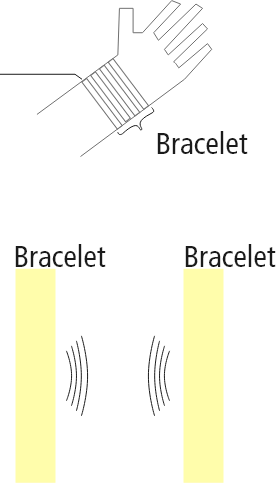
\includegraphics[scale=0.4]{images/projectideas/bracelt.png}
        \caption{Shows the bracelt concept.}
        \label{fig:braceltIdea}
    \end{figure}

    \subsubsection{Music controll Jacket}
    \begin{flushleft}
        Another idea was to develop a jacket that can be used to change a song you are listening on a phone. Therefore,
        strips are placed on the left or right arm that can be used to change the song to make it louder or to stop the song, 
        for example (see Figure ~\ref{fig:jacketIdea}).
    \end{flushleft}

    \begin{figure}[h!]
        \centering
        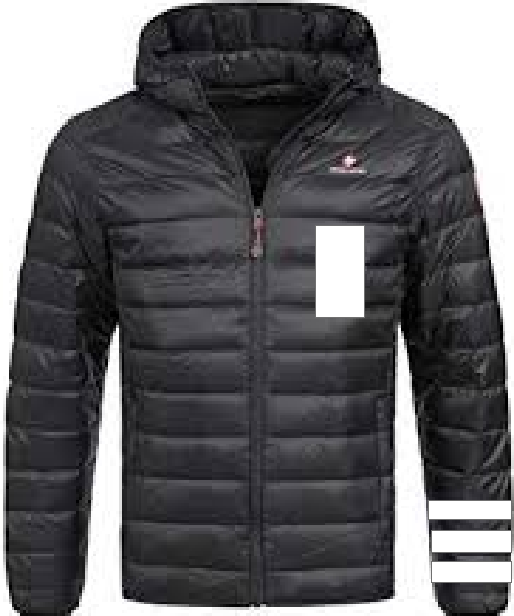
\includegraphics[scale=0.2]{images/projectideas/jacket.png}
        \caption{Shows the concept of a jacket with interaction constraints.}
        \label{fig:jacketIdea}
    \end{figure}

    %why is the new chapter before image? 
    \subsubsection{Blossom shaped Lamp}
    \label{BlossomShapedLamp}
    \begin{flushleft}
        A third and last idea is about lightness. The idea is to build a lamp of a blossom that can be modified by the user.
        Every blossom leaf has a magnet inside, so it is possible to connect each leave. If some leaves are connected, the lamp that 
        is in the middle of the flower blossom changes its color. Moreover, it is possible to rotate the whole lamp and to change the
        brightness by an analog switch (see Figure ~\ref{fig:blossomLamp}).
    \end{flushleft}

    \begin{figure}[h!]
        \centering
        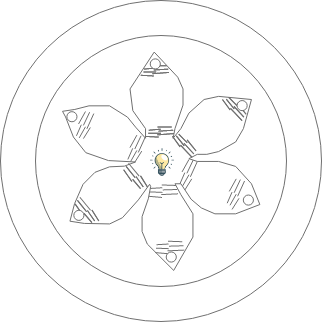
\includegraphics[scale=0.4]{images/projectideas/blossomLamp.png}
        \caption{Shows the concept of a blossom shaped lamp.}
        \label{fig:blossomLamp}
    \end{figure}

    \subsection{Detailed Explaination of the Idea}
        \begin{flushleft}
            At the end, we dicided to develop the third idea (see chapter \ref{BlossomShapedLamp}). That's why, we want to explain 
            how it should work in detail. \newline
            The base of the prototyp will be milled, so we get a perfect shape of the the base. Therefore, we will use Autodesk Fusion 360\cite{autodeskFusion360}
            to model it. in teh center of the base will be the blossom shaped lamp that can be opened. Around this, we want to have a 
            circled shaped groud. There we want to place cupper foil that is linked with a microcontroller, % add explaination
            so the foil ca be used as a slider. This interaction will change the brightness of the lamp. \newline
            However, the major functionality is the lamp itself. Therefore, we want to laser cut the shape, so the users of the lamp can
            take one or several blossoms to open it. This will change the color shining of the lamp. We want to use a transparent acrylic glass.
            Therfore, we have to cut holes inside the glass, so the shape can change.  \newline
            If all blossoms are connected, then the lamp doesn't shine at all. However, if the user open the blossom, then the lamp gets on
            and the color change. 
            \newline
            \newline
            To develop such a device, we want to use an Arduino Pro Mini, copper foil and programmable WS2812B leds.
            A three-dimensional model of the base can be found in Figure ~\ref{fig:blossomBaseModel}
            
            \begin{figure}[h!]
                \centering
                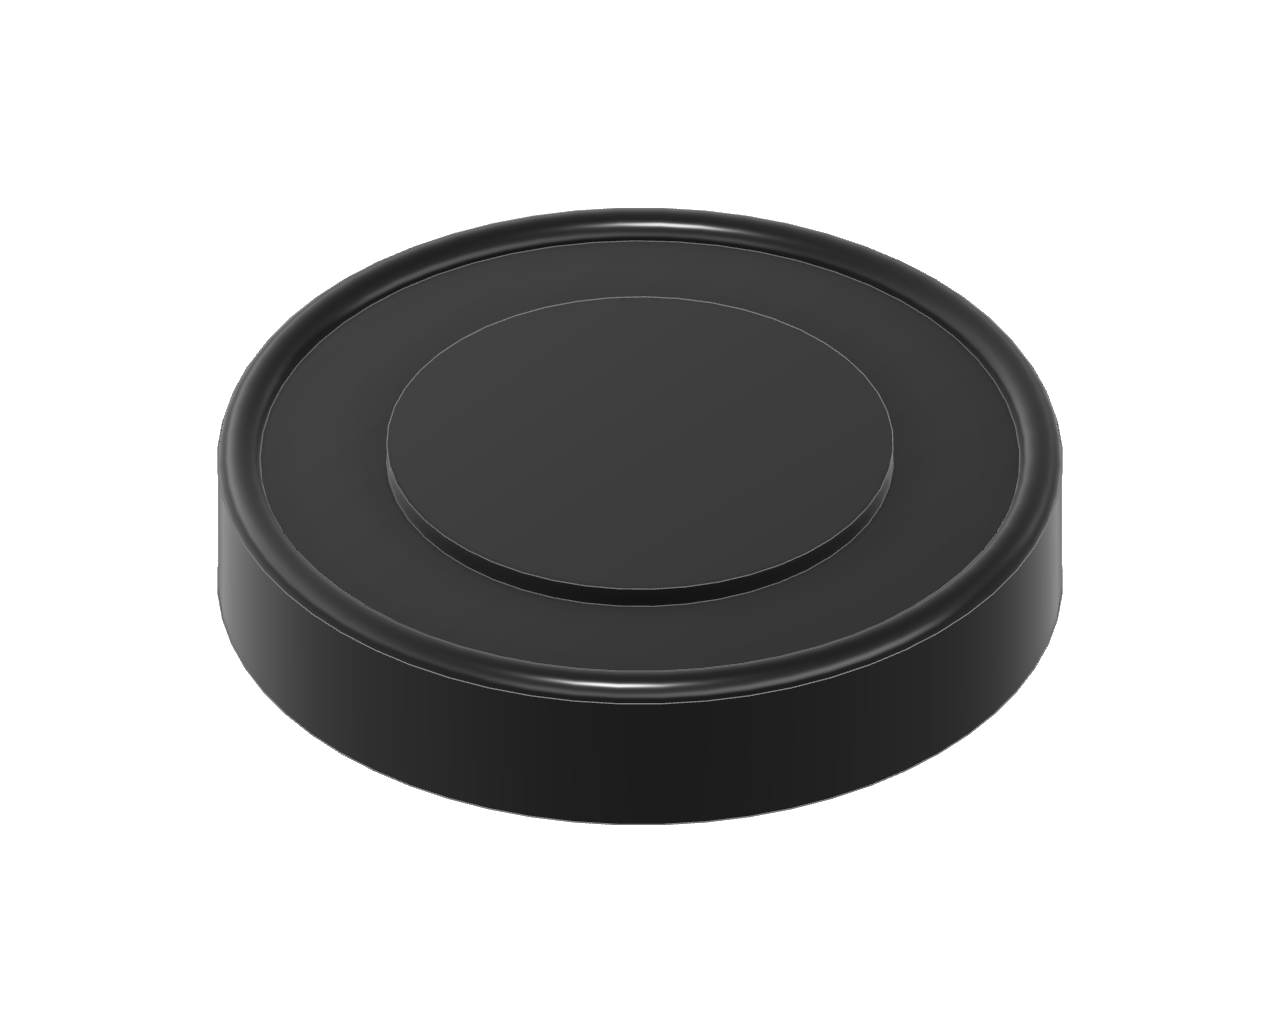
\includegraphics[scale=0.3]{images/process/FlowerLamp.png}
                \caption{Shows a three-dimensional base model of the blossom lamp idea.}
                \label{fig:blossomBaseModel}
            \end{figure}
        \end{flushleft}

    \subsection{Building Process}
        \begin{flushleft}
            To build the prototyp, we modeled the base for the lamp (see Figure ~\ref{fig:blossomBaseModel}). Therfore, we used
            Autodesk. After doing so, we used a milling machine. We only had to convert the 3D model into a .iges file.
            The result of the milling process can be seen in Figure ~\ref{fig:blossomBase}.
        \end{flushleft}

        \begin{figure}[H]
            \centering
            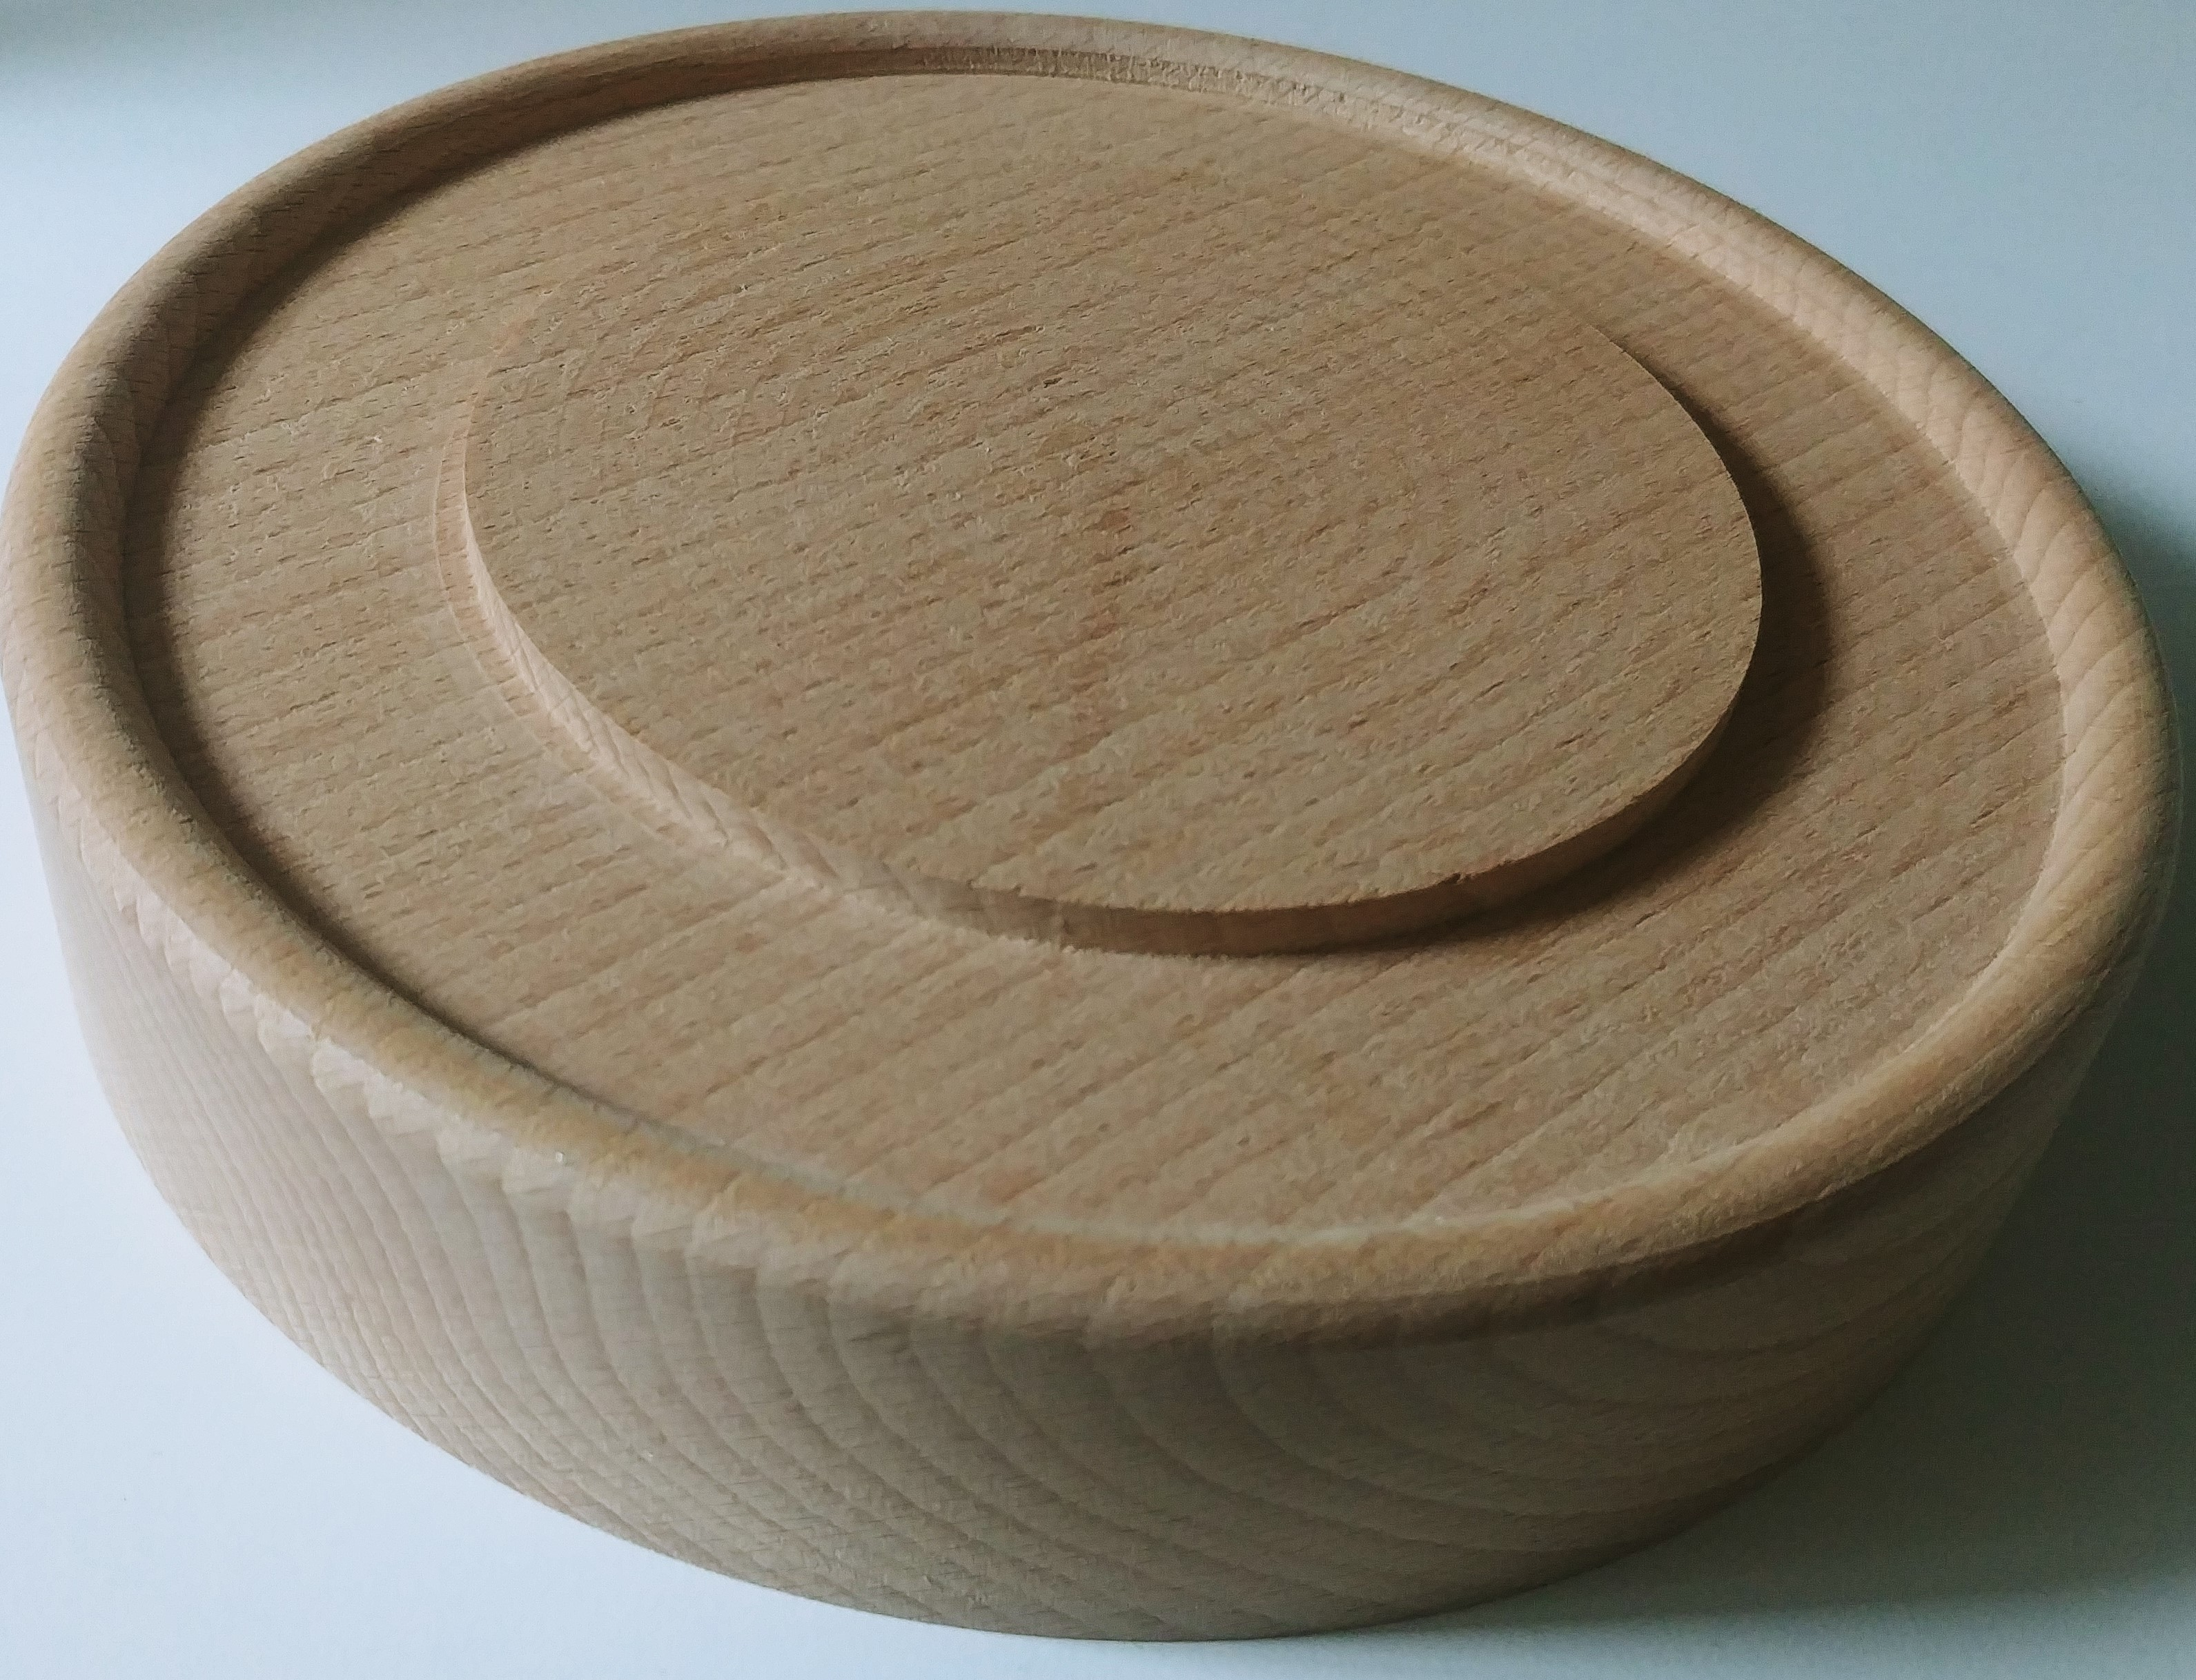
\includegraphics[scale=0.05]{images/process/base.jpg}
            \caption{Shows the base that has been milled.}
            \label{fig:blossomBase}
        \end{figure}
        \noindent
        After milling the base, we had to experiment with the lase cuter and how big the holes and the distance between them 
        should be, so we can laser cut the blossom shape later. To laser cut everything, we used Illustator\cite{illustrator} and a laser cutter. 
        With Illustator we can design the shape that has to be cut. Therfore, we tried a width of 1mm, 0.75mm and 0.5mm and a distance
        of 1mm, 0.75mm, 0.5mm. The result can be found in Figure ~\ref{fig:01_LaserCut}.\\
        \noindent
        After doing the first tried we decided to work with wood because it is more flexible 
        than acrylic glas (see Figure ~\ref{fig:03_LaserCut} and ~\ref{fig:04_LaserCut}).

        \begin{figure}[H]
            \centering
            \begin{subfigure}{.45\textwidth}
              \centering
              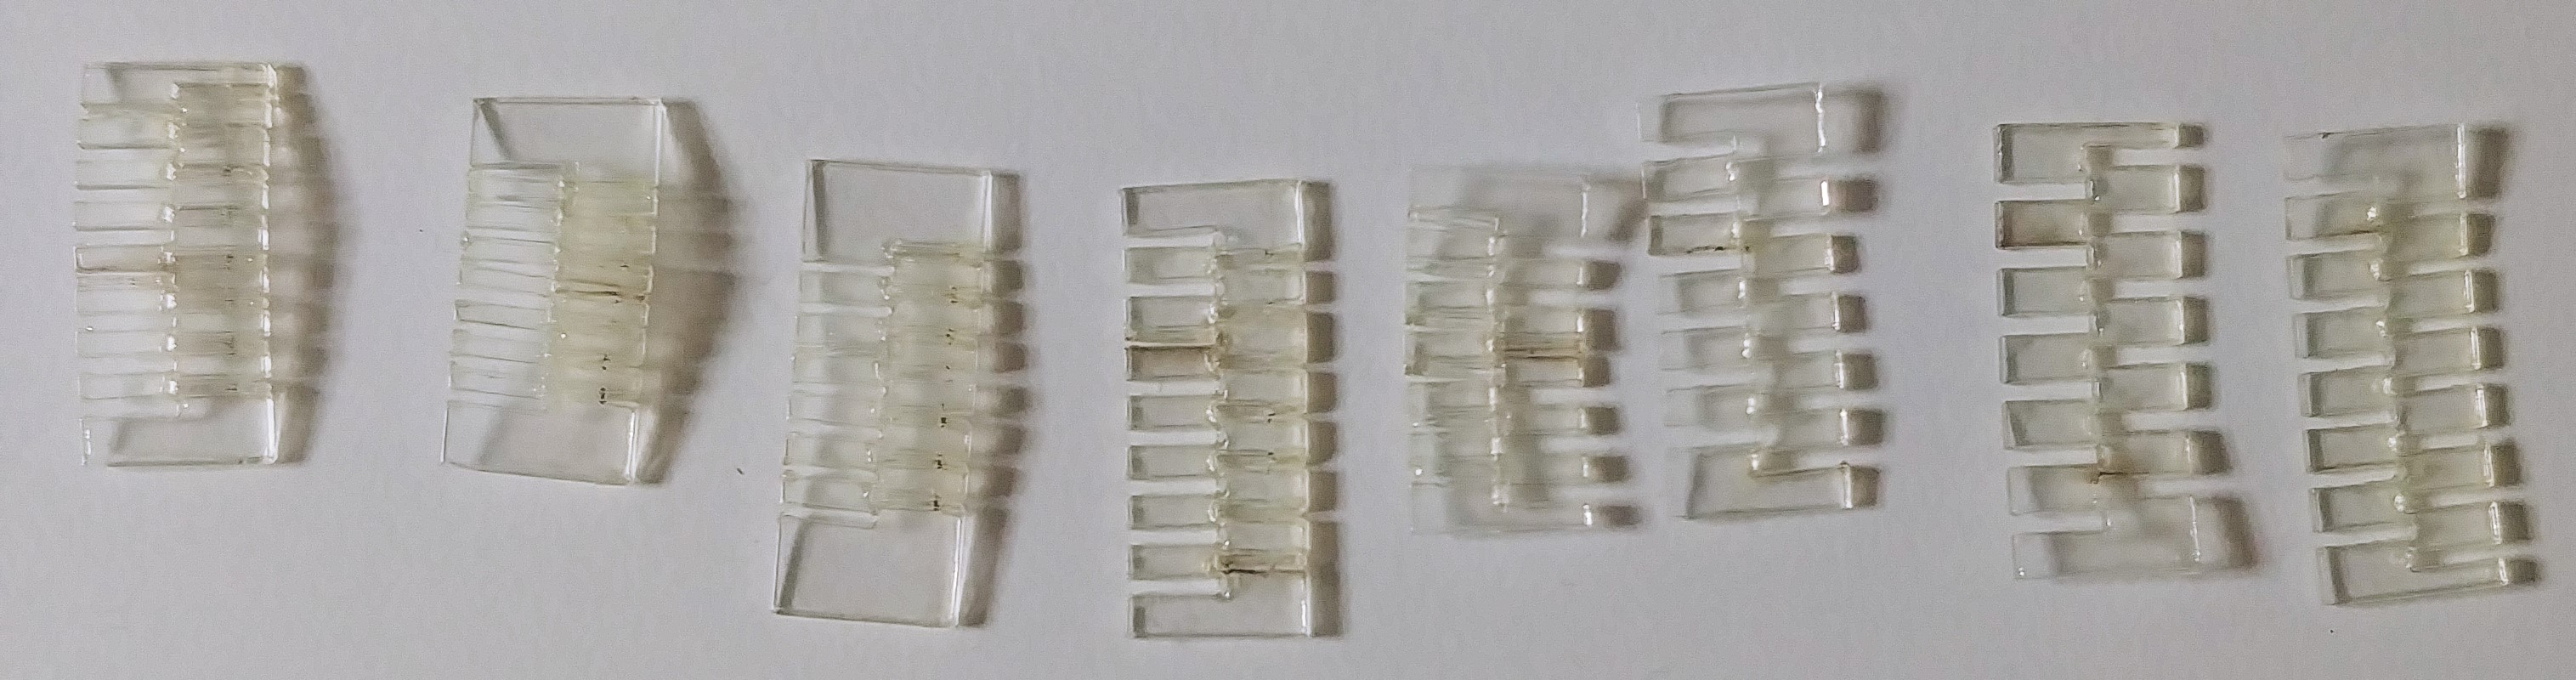
\includegraphics[width=0.8\linewidth]{images/process/01_LaserCut.jpg}
              \caption{Shows the first try to laser cut in general, so we wanted to
                       find out what distances of the wholes and how big the wholes 
                       should be in general.}
              \label{fig:01_LaserCut}
              \vspace{6mm}
            \end{subfigure}
            %\hfill
            \hspace{1mm}
            \begin{subfigure}{.45\textwidth}
                \centering
                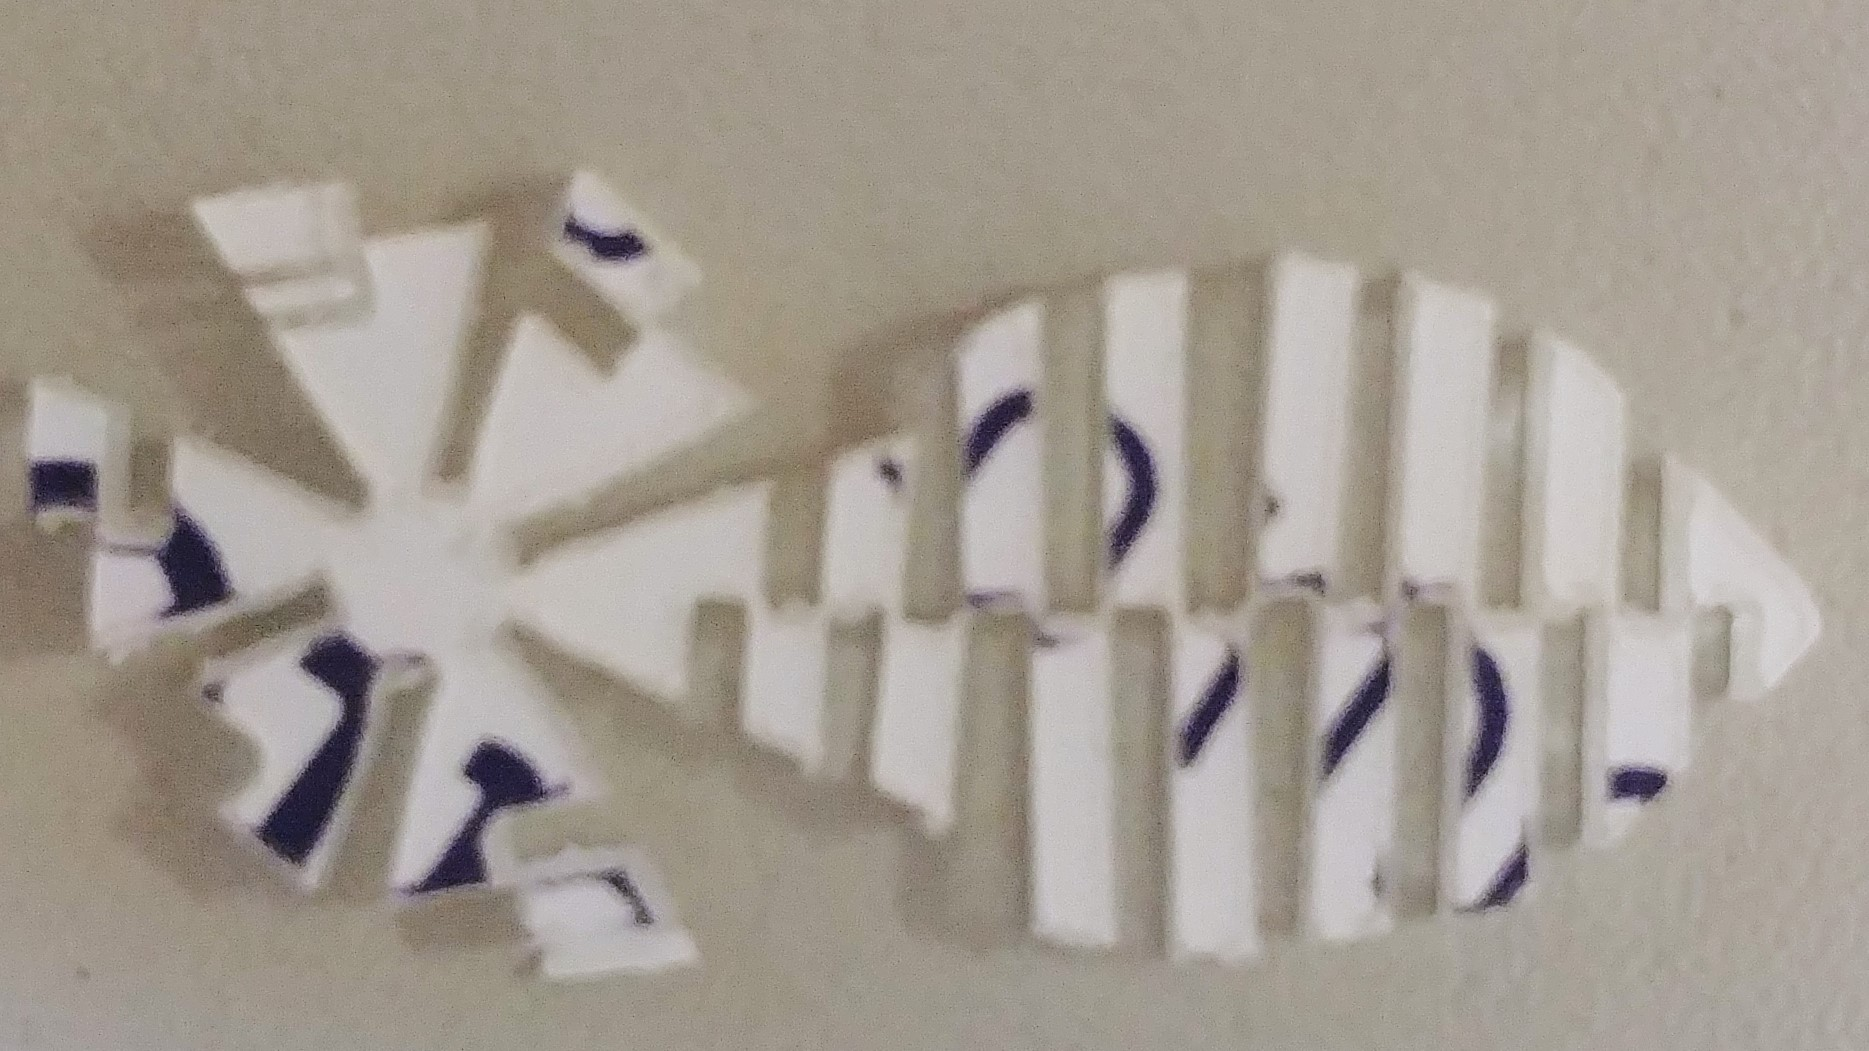
\includegraphics[width=0.8\linewidth]{images/process/02_LaserCut.jpg}
                \caption{Shows the second try to laser cut the shape. This time we have been
                         working with acrylic glass that was 2mm thin. The wholes are 1mm thick 
                         and the distance between those are only 5mm. When we tried to move
                         the parts, they broke.}
                \label{fig:02_LaserCut}
                \vspace{6mm}
            \end{subfigure}
            %\hfill
            \hspace{1mm}
            \begin{subfigure}{.45\textwidth}
                \centering
                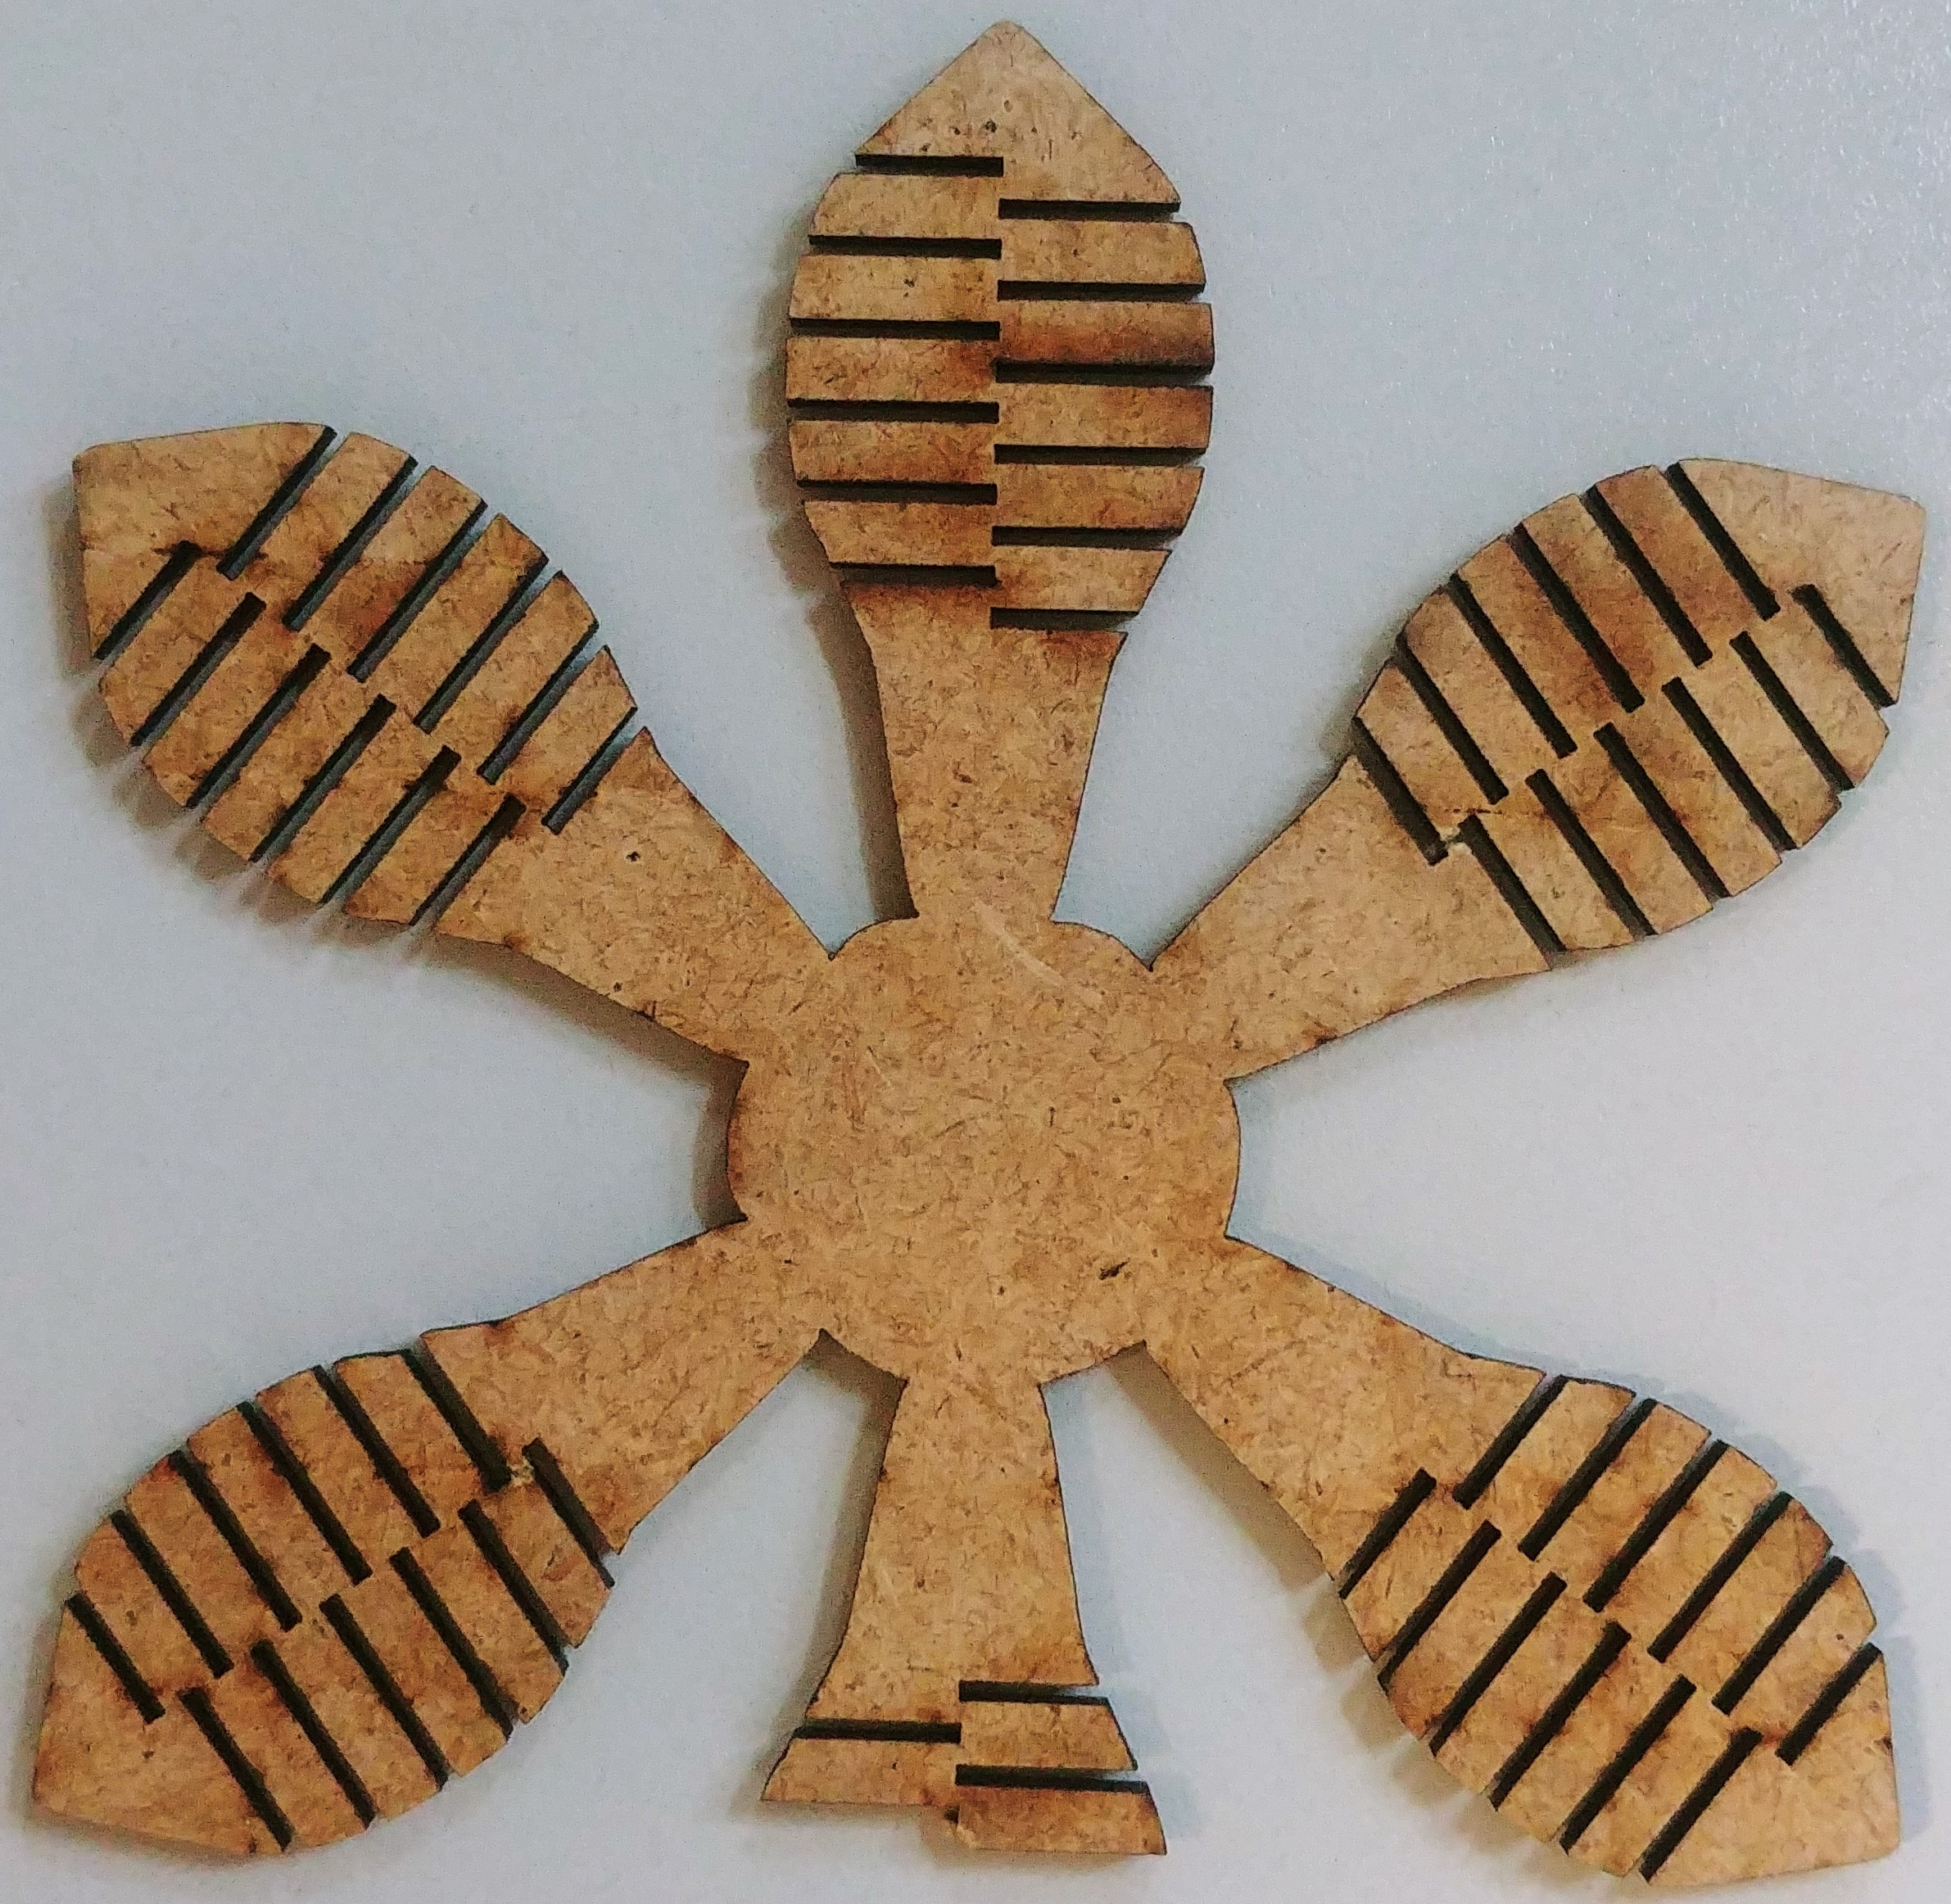
\includegraphics[width=0.8\linewidth]{images/process/03_LaserCut.jpg}
                \caption{Shows the third try to laser cut the shape. This time we have been
                         working with wood plate what is 3mm thin. The wholes are 1mm thick 
                         and the distance between those are only 5mm. When we tried to move
                         the parts, they broke.}
                \label{fig:03_LaserCut}
                \vspace{6mm}
            \end{subfigure}
            %\hfill
            \hspace{1mm}
            \begin{subfigure}{.45\textwidth}
                \centering
                \includegraphics[width=0.8\linewidth]{images/process/04_LaserCut.jpg}
                \caption{Shows the fourth try to laser cut the shape. This time we have been
                         working with MDR 1mm thin plate. The wholes are 0.5mm thick and the 
                         distance between those are only 2.5mm, so they broke.}
                \label{fig:04_LaserCut}
                \vspace{6mm}
            \end{subfigure}
            \caption{Shows ring design.}
            \label{fig:laserCutTests}
        \end{figure}
        \noindent

    \subsection{Implementation Process}
        \begin{flushleft}
            After cutting everything we soldered everything. Therefore, we used an Arduino Pro Mini \cite{arduinoProMini} 
            as an microcontroller, some resistors (10k\si{\ohm}), copper foil and an rgb-strip. \newline
            The resistors and the copper foil are used to build an capacitive sensor. \cite{Badger2019} 
            This means, they can detect finger touching and it will be used to create a analog slider.
            The rgb-strip will be used to make the lamp shine in different colors. \cite{Burgess2019} 
            \newline 
            \noindent
            To program these functionalities, we programmed an Arduino program that can deal with these input 
            and output. The final code can be found on GitHub. %TODO: Add right webpage
        \end{flushleft}

        % has to be changed later
        \begin{figure}[h!]
            \centering
            \begin{subfigure}{.5\textwidth}
            \centering
            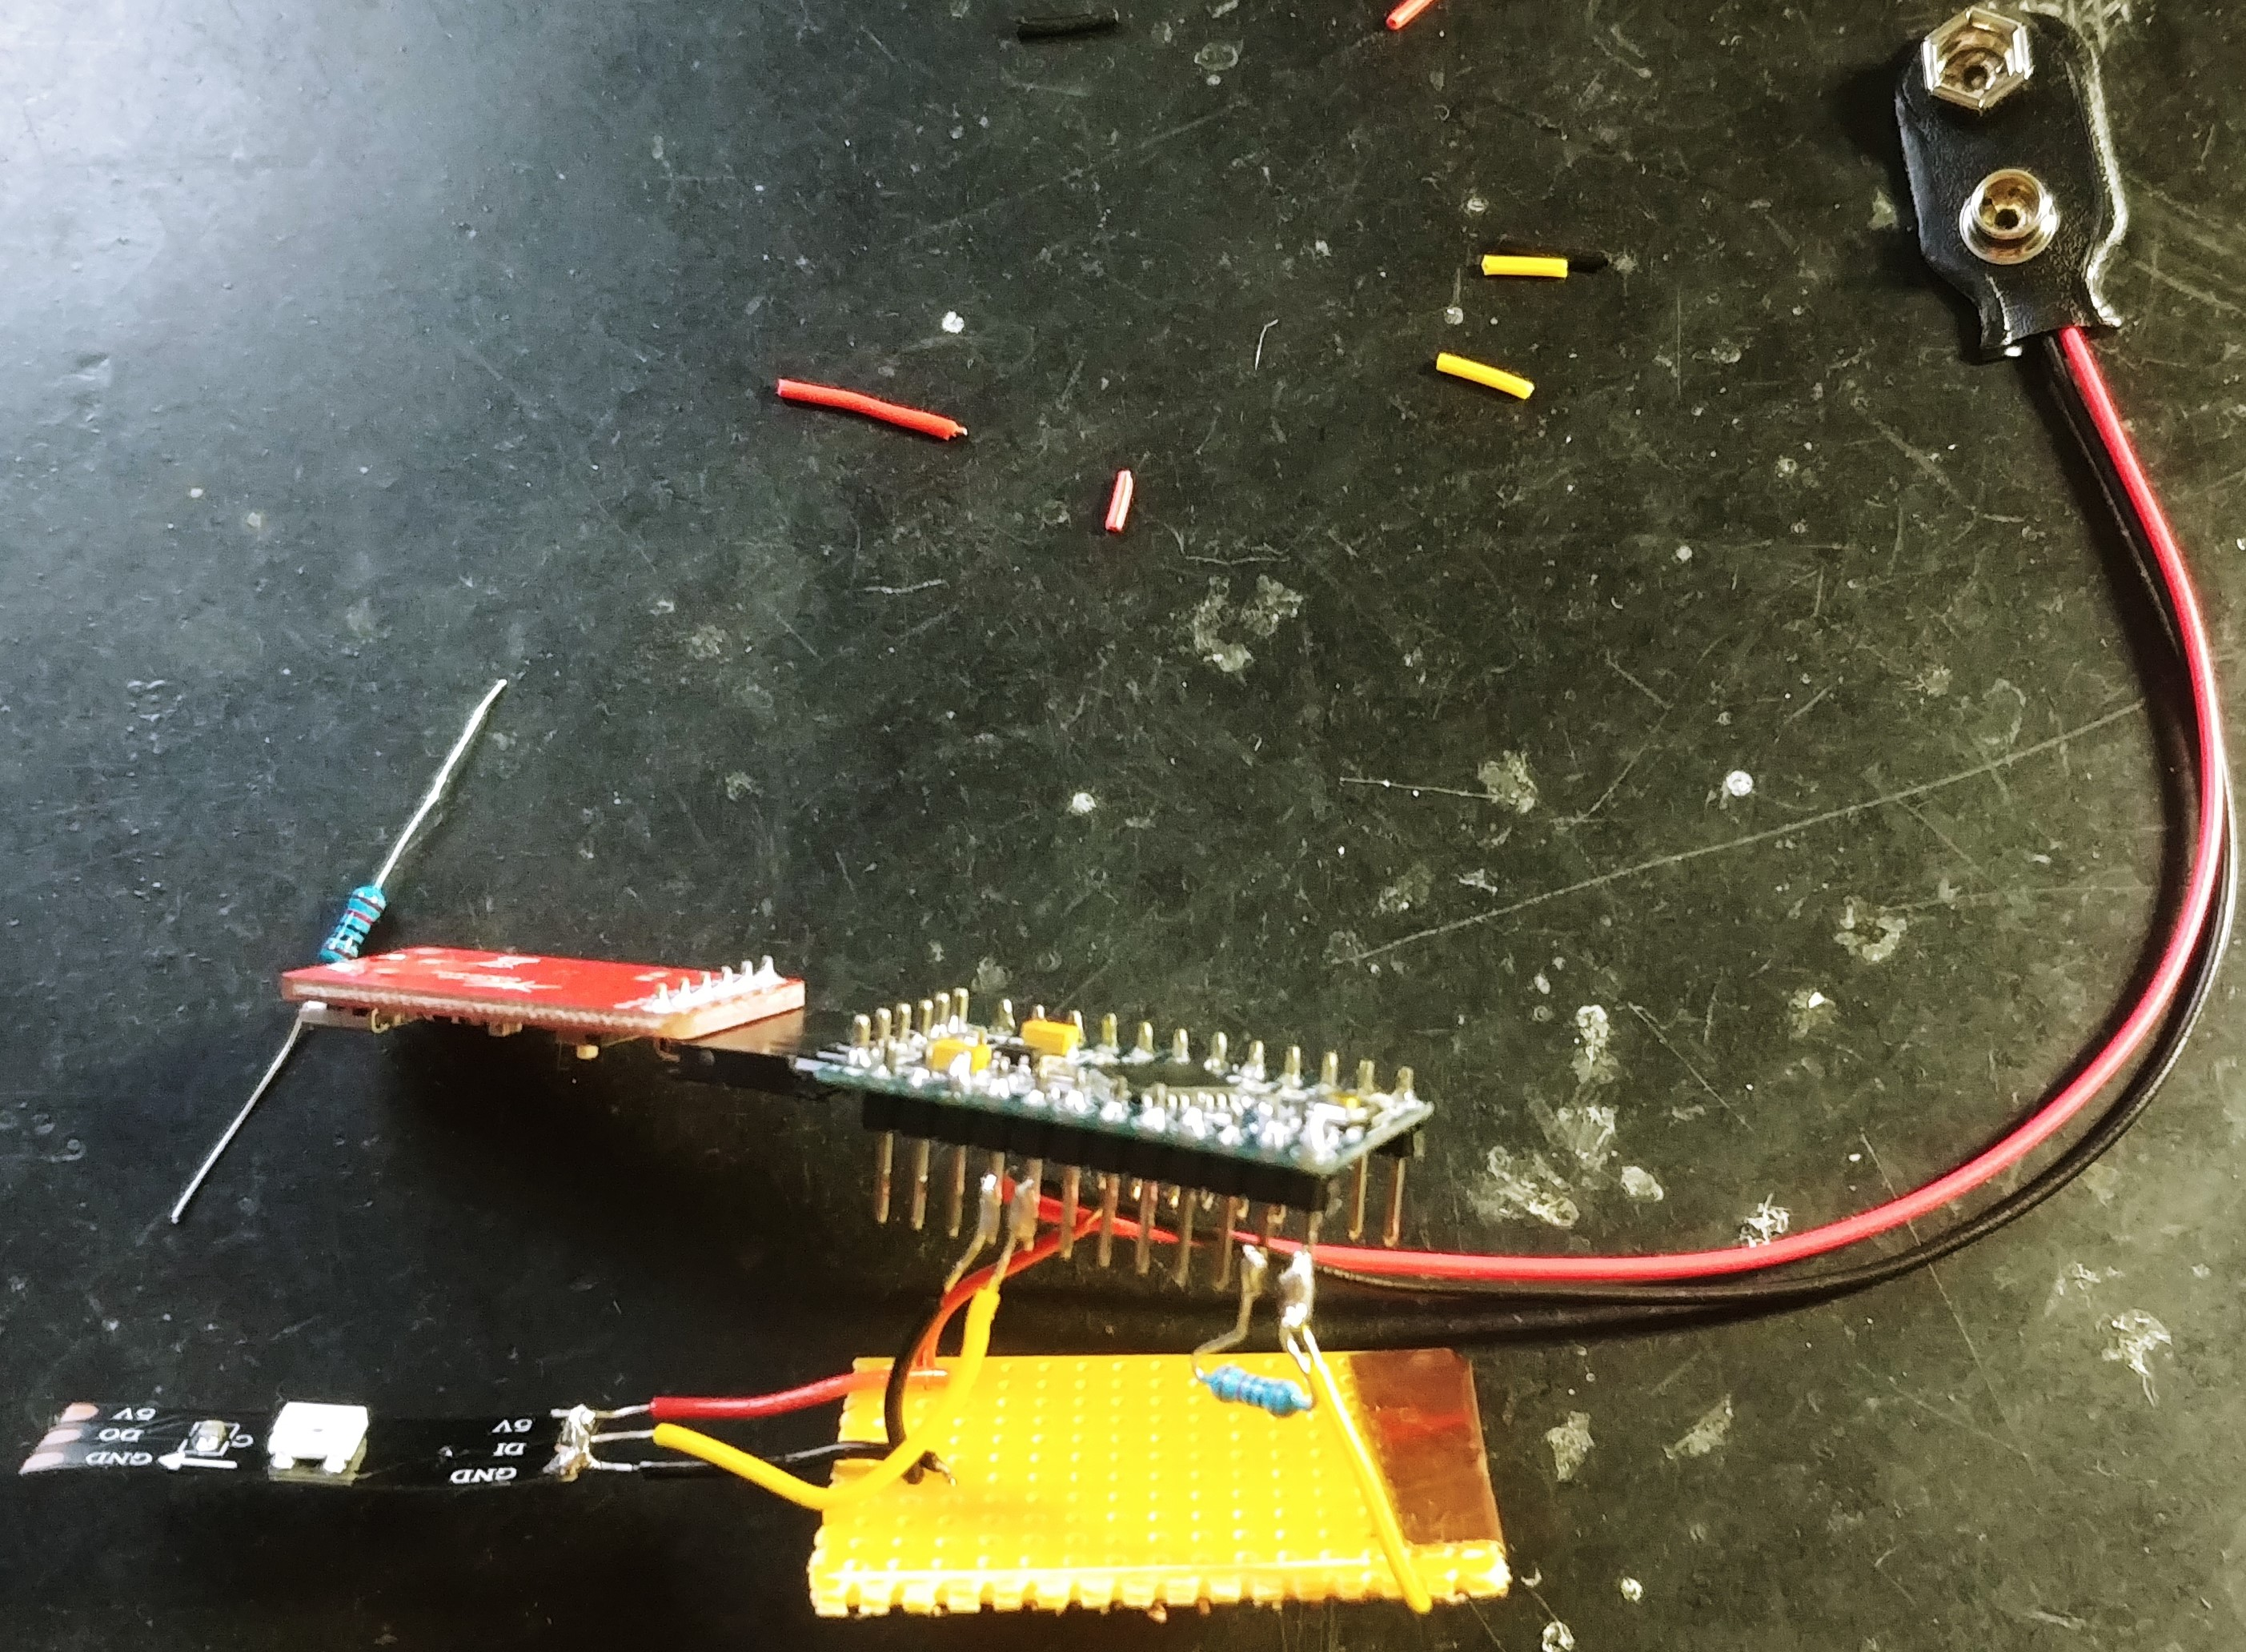
\includegraphics[width=.8\linewidth]{images/process/solderingProcess.jpg}
            \caption{Shows the soldering process of the project to test the functionality.}
            \label{fig:test_shapes}
            \end{subfigure}%
            \begin{subfigure}{.5\textwidth}
            \centering
            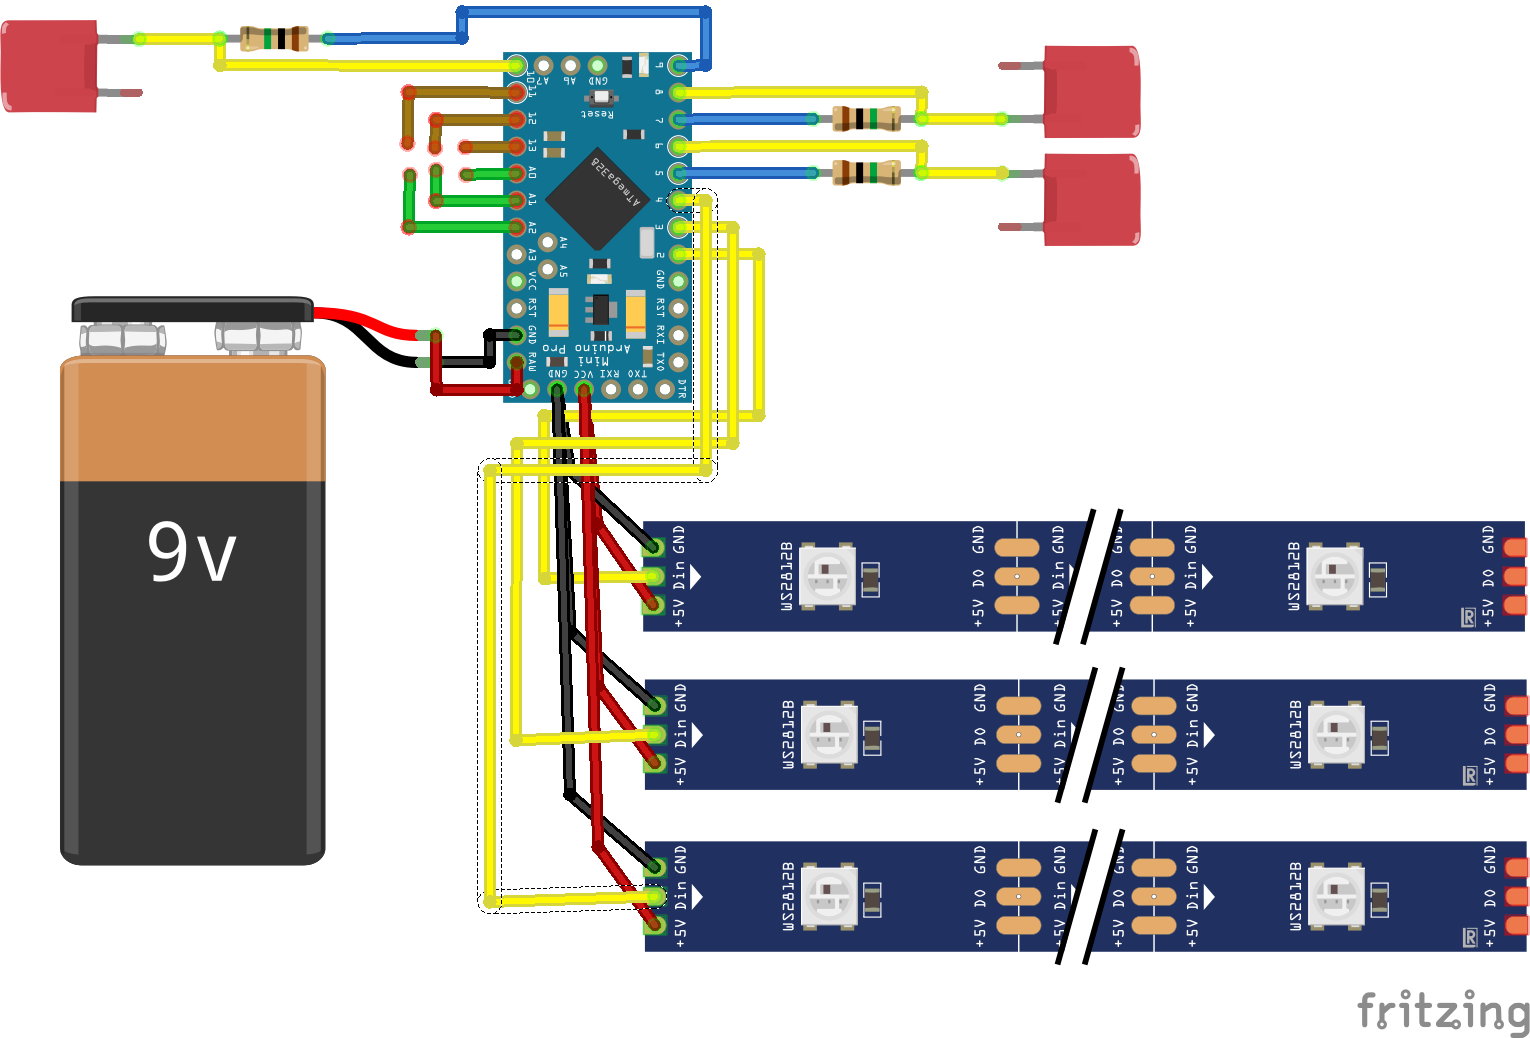
\includegraphics[width=.8\linewidth]{images/process/sensorLinks.png}
            \caption{Shows the links between the microcontroller and the leds and copper foil that is 
            used as a capacitive sensor. This image has been done by Frizing. \cite{fritzing}}
            \label{fig:ringdesign2}
            \end{subfigure}
            \caption{Shows the soldering process and linking.}
            \label{fig:laserCutTests}
        \end{figure}

    \subsection{Merging Code and Physical Components}
        \begin{flushleft}
            After coding everything and testing the code if everything is working like we wanted, we glued
            the blossom and the base together and connected the copper foil to the base. The result can be 
            seen in Figure ~\ref{fig:finalPrototyp}.
        \end{flushleft}

        \begin{table}[h!]
            \centering
            \begin{tabular}{c}
              \centering
              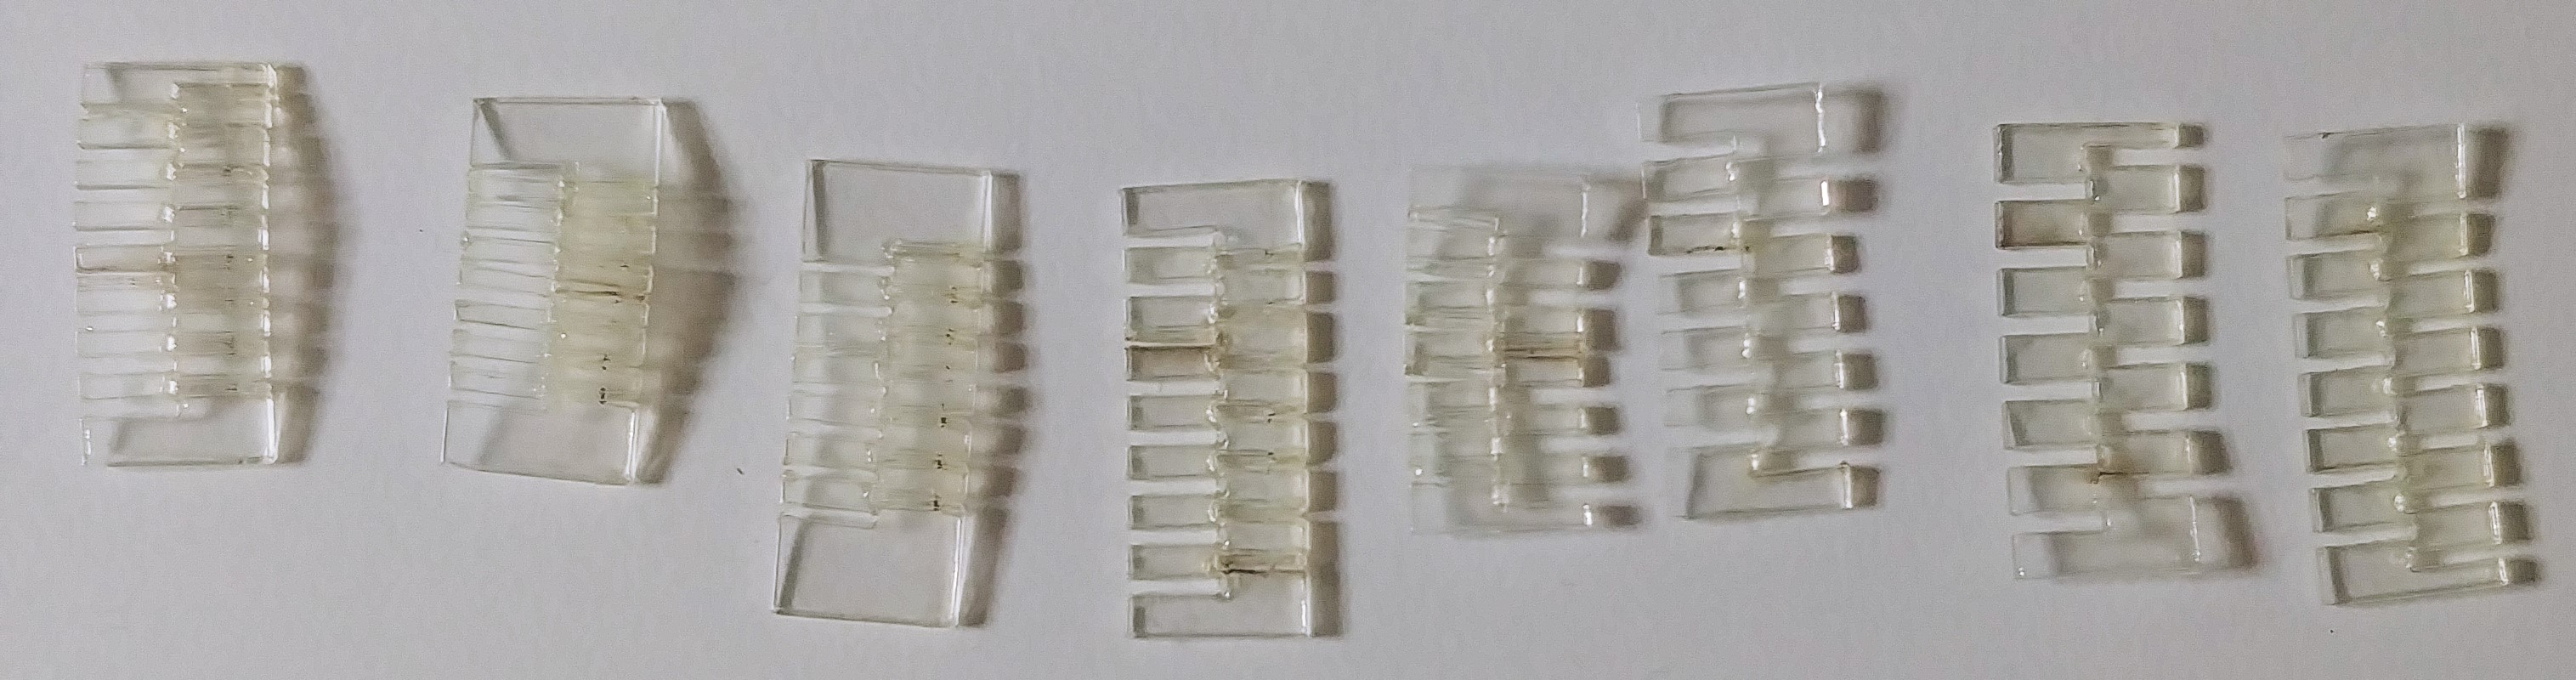
\includegraphics[width=.8\linewidth]{images/process/01_LaserCut.jpg}
            \end{tabular}
            \caption{Shows the final prototyp of the blossom shaped lamp}
            \label{fig:finalPrototyp}
        \end{table}
\end{document}